\iffalse
\let\negmedspace\undefined
\let\negthickspace\undefined
\documentclass[journal,12pt,onecolumn]{IEEEtran}
\usepackage{cite}
\usepackage{amsmath,amssymb,amsfonts,amsthm}
\usepackage{algorithmic}
\usepackage{graphicx}
\usepackage{textcomp}
\usepackage{xcolor}
\usepackage{txfonts}
\usepackage{listings}
\usepackage{enumitem}
\usepackage{mathtools}
\usepackage{gensymb}
\usepackage{comment}
\usepackage[breaklinks=true]{hyperref}
\usepackage{tkz-euclide} 
\usepackage{listings}
\usepackage{gvv}                                        
\def\inputGnumericTable{}                                 
\usepackage[latin1]{inputenc}                                
\usepackage{color}                                            
\usepackage{array}                                            
\usepackage{longtable}                                       
\usepackage{calc}                                             
\usepackage{multirow}                                         
\usepackage{hhline}                                           
\usepackage{ifthen}                                           
\usepackage{lscape}

\newtheorem{theorem}{Theorem}[section]
\newtheorem{problem}{Problem}
\newtheorem{proposition}{Proposition}[section]
\newtheorem{lemma}{Lemma}[section]
\newtheorem{corollary}[theorem]{Corollary}
\newtheorem{example}{Example}[section]
\newtheorem{definition}[problem]{Definition}
\newcommand{\BEQA}{\begin{eqnarray}}
 \newcommand{\EEQA}{\end{eqnarray}}
\newcommand{\define}{\stackrel{\triangle}{=}}
\theoremstyle{remark}
\newtheorem{rem}{Remark}
\begin{document}
 \bibliographystyle{IEEEtran}
 \vspace{3cm}
 \title{\textbf{10.5.2.11}}
 \author{EE23BTECH11048-Ponugumati Venkata Chanakya$^{*}$% <-this % stops a space
 }
 \maketitle

 \bigskip
 \renewcommand{\thefigure}{\theenumi}
 \renewcommand{\thetable}{\theenumi}
 \textbf{QUESTION:}
 The 17th term of ap exceeds its 10th term by 7. FInd its common difference?\\
 \solution
\fi
 \begin{align}
     x(n) &= \{x(0)+nd\}u(n) \label{eq 10.5.2.11_1}\\
     x(17)-x(10) &= 7\\
    \implies {x(0)+17d}-{x(0)+10d} &= 7\\
    \implies 17d-10d &= 7\\
    \implies 7d &= 7\\
    \implies d &= 1
 \end{align}

 
 \begin{table}[!ht]
    \centering
        
      \begin{tabular}{|c|c|c|} 
      \hline
\textbf{Variable}& \textbf{Description}& \textbf{Value}\\\hline
         $x(n)$& $n^{th}$ term of AP&none\\\hline
          $d$&common difference between the terms of AP&none\\\hline
          $x(17)-x(10)$& difference of $17^{th}$  and $10^{th}$ term of X &$7$ \\ \hline
         
    \end{tabular}

    \caption{input parameters}
    \label{tab:10_5_2_11}
\end{table}
Taking Z-Transform:
\begin{enumerate}
    \item $\mathcal{Z}\{u(n)\}$
\begin{align}
    u(n) \system{Z} \frac{1}{1-z^{-1}} \{\abs{z} > 1\} \label{eq 10.5.2.11_7}
\end{align}
    \item $\mathcal{Z}\{nu(n)\}$ 
\begin{align}
    nu(n) \system{Z} \frac{z^{-1}}{(1-z^{-1})^2}\, \{\abs{z} > 1\} \label{eq 10.5.2.11_8} 
\end{align}0
Taking Z-Transform of \eqref{eq 10.5.2.11_1} using \eqref{eq 10.5.2.11_7}and \eqref{eq 10.5.2.11_8}
\begin{align}
    X(n)=100\frac{1}{1-z^{-1}} +\frac{z^{-1}}{(1-z^{-1})^2}\
\end{align}
\end{enumerate}
Let \\
\begin{align}
x(n)&= \lbrace 101,102,103,...\rbrace 
\end{align}
\begin{figure}
    \centering
    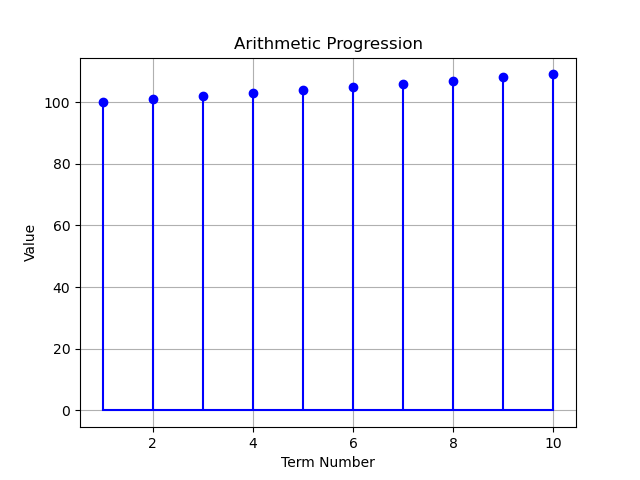
\includegraphics{ncert-maths/10/5/2/11/figs/fig1.png}
    \caption{ }
    \label{fig:x(n) }
\end{figure}
 
 %\end{document}
